\documentclass[a4paper, 12pt]{article}
\usepackage[lmargin=2.5cm, 
			rmargin=2.5cm, 
			tmargin=2cm, 
			bmargin=2.5cm]{geometry}

\usepackage[utf8]{inputenc}
\usepackage[OT2, T1]{fontenc}
\usepackage[english, serbian]{babel}
\usepackage[none]{hyphenat}

\usepackage{amsfonts, amssymb, amsmath, amstext}
\usepackage{graphicx, wrapfig, enumitem, hyperref, gensymb}
\usepackage{chngcntr, ragged2e, pgfplots}
\usepackage{caption, float, lmodern, cleveref}

\pgfplotsset{compat=1.14}
\floatstyle{plaintop}
\newfloat{grafik}{tbph}{loc}
\floatname{grafik}{Grafik}
\crefname{grafik}{grafik}{grafici}
\Crefname{grafik}{Grafik}{Grafici}

\counterwithout{enumi}{section}

\title{Projekat iz primene senzora i aktulatora}
\author{Vladimir Galović i Stefan Ostojić}
\date{\today}

\begin{document}

\begin{titlepage}

\begin{figure}
\centering
\vspace*{-2cm}

\includegraphics[scale=0.56]{images/ftnLogo}
\label{fig:ftn_logo}
\end{figure}

\vspace*{2cm}

\begin{center}
\begin{Large}
\textbf{PROJEKAT IZ PRIMENE SENZORA I AKTUATORA}
\end{Large}
\end{center}

\vspace{1.5cm}

\begin{table}[H]
\def \arraystretch{1.25}

\setlength\parindent{16pt}
\textbf{NAZIV PROJEKTA:}\\[7pt]
\begin{tabular}{|p{16cm}|}
\hline
\setlength\parindent{10pt}
Regulator temperature i vlažnosti vazduha\\
\hline
\end{tabular}

\vspace{0.5cm}

\textbf{TEKST ZADATKA:}\\[7pt]
\begin{tabular}{|p{16cm}|}
\hline
\setlength\parindent{10pt}
Čitanje i kontrolisanje temperature i vlažnosti vazduha u zatvorenoj sredini.\\
\hline
\end{tabular}

\vspace{0.5cm}

\textbf{MENTOR PROJEKTA:}\\[7pt]
\begin{tabular}{|p{16cm}|}
\hline
\setlength\parindent{10pt}
Prof. Jovan Bajić\\
\hline
\end{tabular}

\vspace{0.5cm}

\textbf{PROJEKAT IZRADILI:}\\[7pt]
\begin{tabular}{|p{16cm}|}
\hline
\setlength\parindent{10pt}
Vladimir Galović (EE 210/2018) i Stefan Ostojić (EE 216/2016)\\
\hline
\end{tabular}

\vspace{0.5cm}

\textbf{DATUM ODBRANE PROJEKTA:}\\[7pt]
\begin{tabular}{|p{16cm}|}
\hline
\setlength\parindent{10pt}
\today \\
\hline
\end{tabular}
\end{table}
\end{titlepage}

\tableofcontents
\pagebreak

\begingroup
\justifying

\section{Uvod}

\vspace{10pt}

Regulacija temperature i vlažnosti vazduha

\vspace{10pt}

\sloppypar
Ova tema je izabrana zbog interesovanja za rad sa DHT22 senzorom dok su sve ostale funkcionalnosti dodate tokom realizacije projekta. Sa ovim snezorom kao prvom tačkom projekta izabran je problem čitanja i regulisanja temperature i vlažnosti vazduha neke zatvorene sredine poput nekog skadišta gde je održavanje temperature i vlažnosti bitno. Primer za ovakav uređaj je humidor za cigare koji održva konstantnu temperaturu (16-22 °C) i vlažnost (60-75 \%) kako bi održao kvalitet cigare (Slika \ref{fig:primer}).

\vspace{10pt}

  Zarad brze i lake realizacije kao osnovna kontrolna jedinica izabrana je Arduiono pltforma koja pruža puno fleksibilnosti. Za aktuator je izabran BLDC motor sa ventilatorom koji bi najbrže uticao na regulisanje temperature i vlažnosti. LCD displej i tastatura su dodate radi lakše interakcije sa korisnikom, a uloga zujalice je da upozori korisnika na prevelike ili premale vrednosti vlažnosti vazduha. 

\vspace{10pt}


Realizacija i upoznavanje sa svim karakteristikama komopnenti je započeta povezivanjem osnovih elemenata na protoboard i Arduino UNO. Pojedinačnim upoznavanjem sa svakom komponentom je smišljen krajni koncept projekta. Kao i ideje za adekvatano testiranje senzora i aktuatora. 

\vspace{10pt}


\begin{figure}[H]
\centering
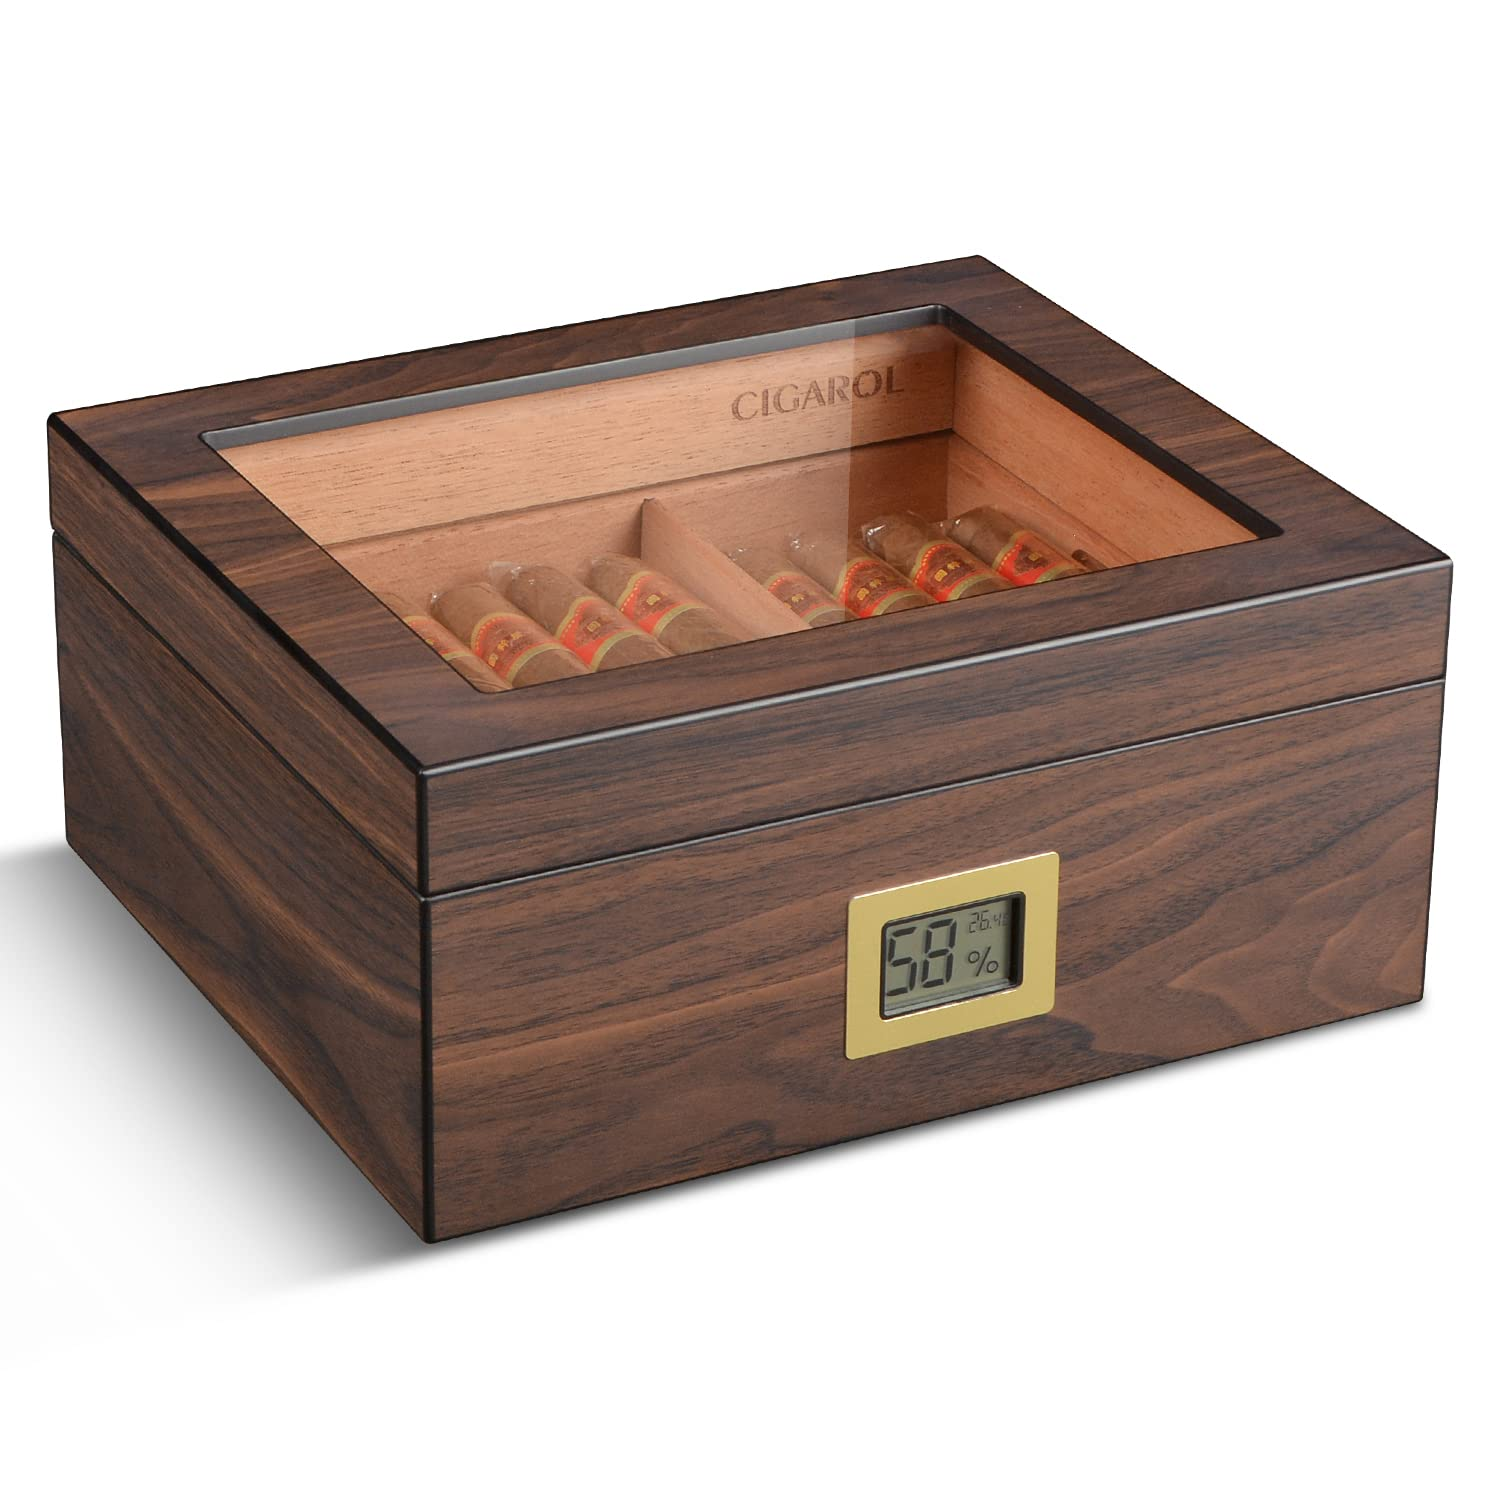
\includegraphics[scale=0.13]{images/primer}
\caption{humidor za cigare} \label{fig:primer}
\end{figure}

\pagebreak
\endgroup

\begingroup
\justifying

\section{Analiza problema}

Regulacija temperature i vlažnosti vazduha neke zatvorene sredine zahteva održanje ove dve vrednosti na prethodno zadatoj konstanti. Humidor održava obe vrednosti veoma precizno čime se kvalitet i ukus cigra ne menja. Da bi to postigao humidor mora imati elemete koji utiču na povećanje i na elemente koji utiču na smanjenje temperature i vlažnosti vazduha. 

\vspace{10pt}

Za povećanje temperature se koriste grejači, a za povećnje vlažnosti vazduha neki izvor vode ili prskalice. Dok za smanjenje i temperature i vlažnosti vazduha se koriste razne vrste ventilatora koji cirkulacijom vazduha smanjuju ove dve vrednosti. Na smanjenje vlažnsti čak utiče i vrsta drveta od koje je humidor napravlje. Kompleksnost nastaje pri delikatnom balansu ove dve celine, povećavanje i smanjivanje temperature i vlažnosti vazduha. Oba segmenta moraju biti proporcionalno aktivni kako bi održali unutrašnjost konstantnom, bez obzira na promene spoljašnje sredine u kojoj se Humidor nalazio.

\vspace{10pt}

\sloppypar
Zarad pojednostavljivanja i lakše realizacije fokus se stavlja samo na proces smanjivanja temperature i vlažnosti vazduha. Za ovaj proces je samo potreban jedan aktuator. Koji je u primeru ovog projekta BLDC motor sa ventilatorom. Dok bi u procesu povećanja temperature i vlažnosti vazduha morali da imam bar dva aktuatora. Grejač i neki sistem vodenih pumpi koji bi distribuitao vodu u odgarajućoj meri. Čime bi se obim i kompleksnost ovog projekta znatno povećao. Ovim pojednostaviljanjem dolazi i do promena merenih vrenosti jer bez dodatnih komponenti naša sredina neće održavati temperaturu i vlažnost kao Hunidor nego kao srednju vrednost prostorije. U tabeli \ref{tab:merne-vrednosti} može se videti razlika između promena mernih vrednost Humidora i ovog projekta.

\vspace{10pt}

\begin{table}[H]
\centering
\begin{tabular}{|l|c|c|}
\hline
& Vlažnost & Temperatura\\
\hline
Humidor & 60 - 75 \% & 16 - 22 °C\\
\hline
Srednja vrednost prostorije & 30 - 80 \% & 26 - 30 °C\\
\hline
\end{tabular}
\caption{Promea merenih vrednosti} \label{tab:merne-vrednosti}
\end{table}

Spajanjem senzora DHT22 i BLDC ventilatora se ostvaruje regulacija temperature i vlažnosti vazduha, iako u suženom obliku. Dok sve ostale komponente doprinose boljoj interakciji korisnika sa uređajom. Regulacija je glavni cilj, dok je interfejs sporedni.

\pagebreak
\endgroup

\begingroup
\justifying
\section{Hardverska realizacija projekta}

\vspace{10pt}

U ovom poglavlju se govori o pojedinačnim komponentama korišćenim u ovom projektu. O njihovim osnovnim karakteristika, prednostima i problemima. Mnoge komponente su izabrane zbog lake dostupnosti, da bi se u slučaju ponovne realzacije ili kavara lako pronašla zamena. Većina komponenti je povezana sa Arduino platformom koja je idealna za realizaciju ovakvih projekata. Glavne prednosti Arduino platforme :

	\begin{itemize}
	
		\item Jednostavnost korišćenja: Arduino je dizajniran da bude jednostavan za upotrebu, čak i za početnike u elektronici i programiranju. Dolazi sa jednostavnom integrisanom razvojnom okolinom (IDE) koja omogućava brzo pisanje, kompajliranje i uploadovanje koda na Arduino mikrokontroler.
		\item Mala veličina: Arduino je veoma kompaktna platforma, što je čini idealnim za ugradnju u razne uređaje i projekte.
		\sloppypar
        \item Niska cena: Arduino pločice su veoma pristupačan, što ga čini odličnim izborom za hobiste, učenike i sve one koji žele da istražuju tehnologiju bez velikih finansijskih ulaganja.
        \item Širok spektar modela: Postoje različiti modeli Arduino pločica, od osnovnih do naprednih, sa različitim brojem ulazno/izlaznih pinova, radnim naponima i drugim karakteristikama. To omogućava korisnicima da odaberu pločicu koja najbolje odgovara njihovom projektu. Za ovaj projekat izabran je Arduino UNO R3 model.
        \item Mogućnost proširenja: Arduino pločice imaju mogućnost proširenja putem širokog spektra dodatnih modula, senzora, aktuatora i drugih komponenti koji se lako povezuju putem standardizovanih interfejsa kao što su digitalni i analogni pinovi, I2C, SPI, UART itd.
        \item Bogata podrška : Arduino ima ogromnu zajednicu korisnika i razvijalaca koji su voljni da dele svoje iskustva, znanje i projekte putem foruma, blogova, YouTube kanala i drugih platformi. Obilje  online resursa drastično olakšava učenje i rešavanje mnogih problema.
        \item Fleksibilnost i prilagodljivost: Arduino se može koristiti za različite svrhe, od jednostavnih projekata poput LED svetla ili automatskog zalivanja biljaka do složenijih projekata kao što su roboti, interaktivne instalacije ili kućna automatizacija. 
       
	\end{itemize}

\vspace{10pt}

\sloppypar
Pored ovoliko prednosti bilo je lako odlučiti se za Arduino okruženje. Neće se ulaziti dataljnije u rad Arduono UNO R3 (Slika \ref{fig:Arduino}) uređaja jer je to van okvira ovog projeta. 

\begin{figure}[H]
\centering
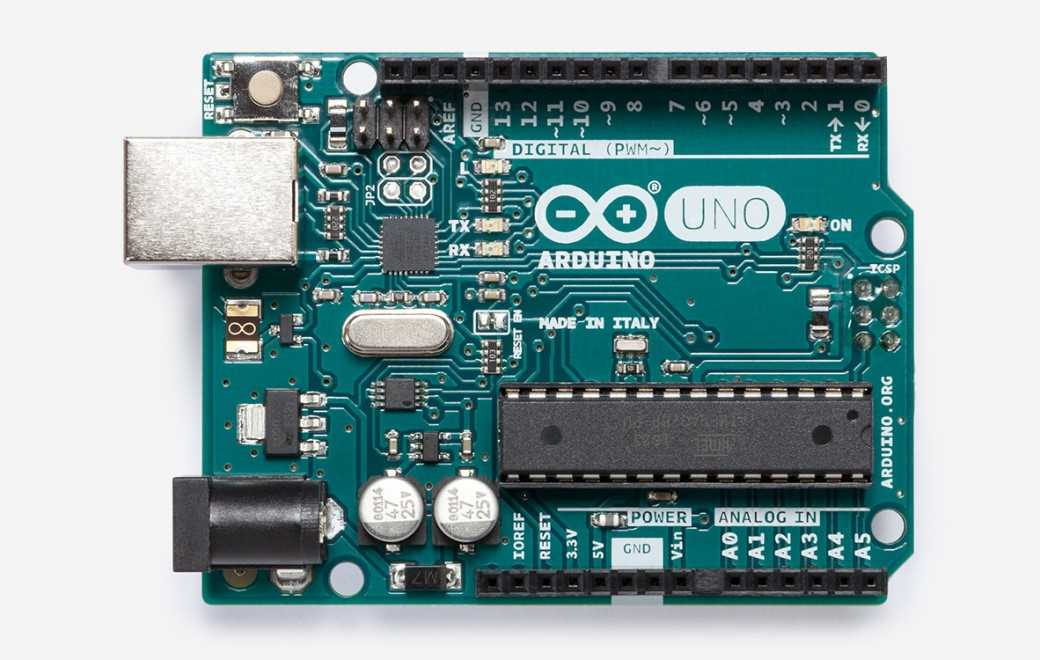
\includegraphics[scale=0.17]{images/ArduinoUNOR3}
\caption{Arduino UNO R3} \label{fig:Arduino}
\end{figure}

\pagebreak


	\subsection{DHT22}

\vspace{10pt}

Kao što je pomenuto u uvodnom delu komponenta koja je inspirisala ovaj projekat je senzor temperature i vlažnosti vazduha DHT22 (Slika \ref{fig:dht22pinssch}). Ovo je glavni senzor u ovom projekt i bilo je od velike važnosti da se izabere relativno precizan i pouzdan senzor. Zato nije izabran možda i više zatupljen senzor DHT11 koji ima manju preciznost. Dimenzije senzora iznose 36x16x9mm (DxŠxV). DHT22 poseduje 3 pina: VCC (5V), DAT (D12) pin i GND. Sve informacije su uzete iz DHT22 datasheet \ref{lib:DHT22-datasheet}. Osnovne karakteristike senzora su:

\begin{figure}[H]
\centering
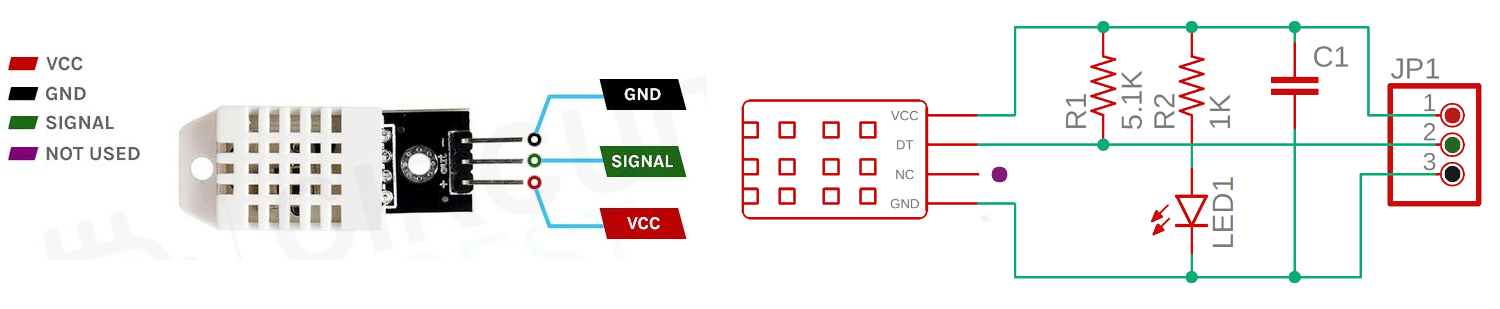
\includegraphics[scale=0.4]{images/dht22pinssch}
\caption{DHT22 senzor i njegov šematik} \label{fig:dht22pinssch}
\end{figure}

\begin{itemize}
	\item Merenje temperature: DHT22 senzor omogućava precizno merenje temperature u opsegu od -40°C do +80°C sa tačnošću od ±0.5°C.
	\item Merenje vlage: Osim temperature, DHT22 senzor takođe meri relativnu vlažnost vazduha u opsegu od 0\% do 100\% sa tačnošću od ±2\%.
	\sloppypar
	\item Digitalni izlaz (8-bit): DHT22 senzor koristi digitalni interfejs za komunikaciju sa mikrokontrolerom, što olakšava integraciju u različite projekte.
	\item Jednostavno korišćenje: DHT22 senzor se lako povezuje sa mikrokontrolerima kao što su Arduino ili Raspberry Pi putem samo tri žice (napajanje, zemlja i digitalni signal).
	\item Pouzdanost: DHT22 senzor je relativno pouzdan i precizan u merenju temperature i vlage, što ga čini popularnim izborom za mnoge aplikacije.
\end{itemize}

\begin{table}[H]
\centering
\begin{tabular}{|l|c|c|c|c|c|}
\hline
& Uslov & Min & Tpično & Max & Jedinica\\
\hline
Napon & DC & 3.3 & 5 & 5.5 & V\\
\hline
Struja & Merena & 1.3 & 1.5 & 2.1 & mA\\
\hline
Struja & Prosečna & 0.5 & 0.8 & 1.1 & mA\\
\hline
Period kolektovanja & Vreme & 1.7 &  & 2 & Sekunde\\
\hline
\end{tabular}
\caption{Električne karakteristike DHT22} \label{tab:DHT22}
\end{table}

Mane ovog senzora: 
\begin{itemize}
\item Brzina odgovora: DHT22 senzor može imati nešto sporiji odgovor u poređenju sa nekim drugim senzorima, što može biti problem u aplikacijama koje zahtevaju brze promene. Što se može videti iz tabele \ref{tab:DHT22}.
\item Osetljivost na kondenzaciju: U uslovima visoke vlažnosti, DHT22 senzor može pokazivati greške zbog kondenzacije vode na površini senzora.
\end{itemize}

\pagebreak

	\subsection{BLDC 5V ventilator (Waveshare fan-4010-5v)}
	
	\vspace{10pt}
	
\begingroup
	
	Glavni aktuator ovog projekta je BLDC ventilator od 5V (Slika \ref{fig:DC40mm5V}). Motor jednosmerne struje bez četkica (BrushLess DC) je izabran zbog njegovih mnogih prednosti u odnosu na klasičan motor jednosmerne struje sa četkicama. Osnovna namena BLDC ventilatora koji je izabran za ovaj projekat je kao hladnjak za Raspberry Pi platformu. Zbog takve namene idealn je izbor za ovaj projekt. Povezanost sa popularnom i standardizovanom Raspberry Pi pltformom olakšava zamenu ovog ventilatora u slučaju njegovog kvara.  Malih je dimenzija zbog čeka se može lako uklopiti u bilo kakav prostor sa lakoćom. Osnovne karakteristike ovog modela su: 

\begin{itemize}
	\item Radni napon: 5V
	\item Snaga: 3.6W
	\item Konekcija: 2 pina
	\item Dimenzije: 40x40x10mm
\end{itemize}

\begin{wrapfigure}{R}{0.5\textwidth}
\centering
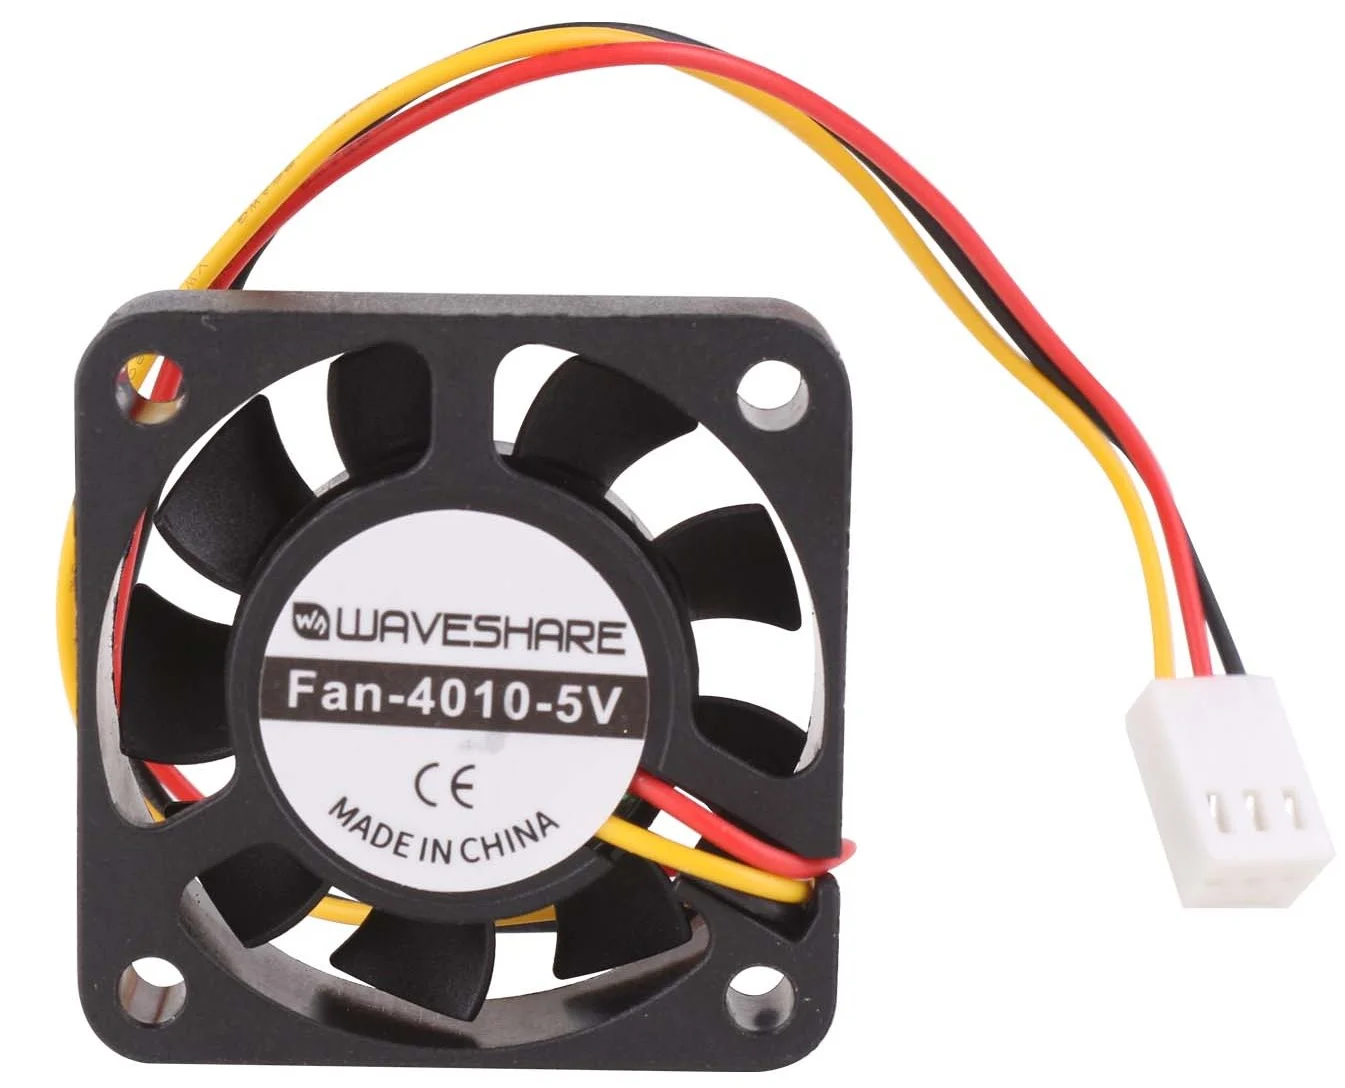
\includegraphics[width=0.5\textwidth]{images/DC40mm5V} 
\caption{Ventilator} \label{fig:DC40mm5V}
\end{wrapfigure}

\vspace{10pt}

Prednosti BLDC motora : 

\begin{enumerate}
	\item Velika brzina obrtanja 
	\item Veliki obrtni momenat 
	\item Odlične startne osobine 
	\item Velika efikasnost 
	\item Rad bez varničenja  
	\item Visoka pouzdanost  
	\item Dug vek eksploatacije
\end{enumerate}

\endgroup
\pagebreak
Jedina mana BLDC motora je složenost elektronske komutacije. Motoru je potrebna i informacija o ugaonom položaju rotora (stalnog magneta) kako bi spoljašnje drajvesko kolo koje vrši komutaciju, donelo odluku kada treba izvršiti preusmeravanje struje kroz namotaje. Praćenje položaja rotor najčešće se vrši primenom Holovih senzora(senzora magnetnog polja).

\vspace{10pt}

Glavni način kontrolisanja BLDC ventilatora u ovom projektu je realizovan korišćenjem  PWM (Pulse Width Modulation) signala (Slika \ref{fig:pwm}) i sa jednim 2N2222A NPN tranzistorom. VCC motora je spojen na 5V a GND motora na kolektor tranzistora. Emiter tranzistora se spaja na GND, a baza na D10 pin Arduina sa kojeg se šalje kontrolni signal. Brzina motora je direktna posledica vrednosti fatkora ispune (odnosom trajanja visokog i niskog naponskog nivoa u toku jedne periode) koji se šalje iz Arduina. Za svaki 1°C povećanja merene vrednosi vrednost faktora ispune se povećava za 20\% sve dok ne dođe do 100\% kada ventilator na maksimalnoj svojoj brzini. 

\vspace{10pt}

\begin{figure}[H]
\centering
	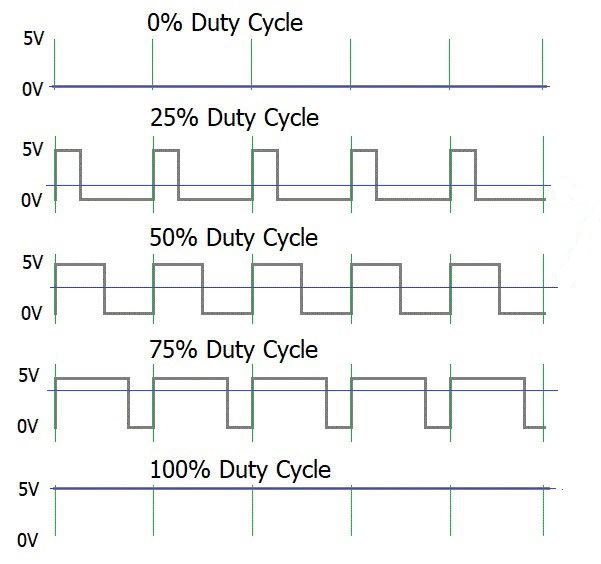
\includegraphics[width=0.7\textwidth]{images/pwm}
	\caption{Primer povećanja faktora ispune u PWM signalu} \label{fig:pwm}
\end{figure}
\pagebreak

	\subsection{Piezo zujalica (MH-FMD)}
	
	Ovaj aktuator (Slika \ref{fig:buzzer}) je dodat kako bi projekat imao još jedan dodatni način interakcije sa korisnikom. Princip rada piezoelektrične zujalice je zasnovan na dovođenju struje na piezo-električni disk koji je spojen sa tankom metalnom pločom. Piezo-električni disk osciluje zbog čega dolazi do savijanja metala napred-nazad. To savijanje metala prouzrokuje zvuk. Obično se koristi kao zvični alarm ili uzbuna. Frekvencija je ono što omogućava piezo zujalicu da proizvede zvuk. Evo nekih karakteristika piezo zujalica:
\begin{itemize}
	\item Što se brže metal savija, to je veći nivo buke koja se proizvodi.
	\item Ova stopa se zove frekvencija.
	\item Što je veća frekvencija, to je veća buka koju čujemo
	\item Opseg radne temperature od -40°C do 85°C
	\item Opseg frekvencije ulazne 2-5kHz (kvadratni signal)
	\item Dimenzije: 32x13x13mm
\end{itemize}

\vspace{10pt}

	Pasivna zujalica korišćena u ovom projektu poseduje 3 pina: VCC (5V), I/O (D11) pin i GND. Neki od nedostataka su ako je potrebna frekvencija van opsega zujalice, i nemogućnost zujanja više zujalica u istom trenutku. Zujalica u ovom projektu ima zadatak da upozori korisnika na problematične vrednosti vlažnosti vazduha koju senzor DHT22 meri. U slučaju ovog projekta to su vrednosti od 30\% kao donja granica i 80\% kao gornja.
	
\begin{figure}[H]
\centering
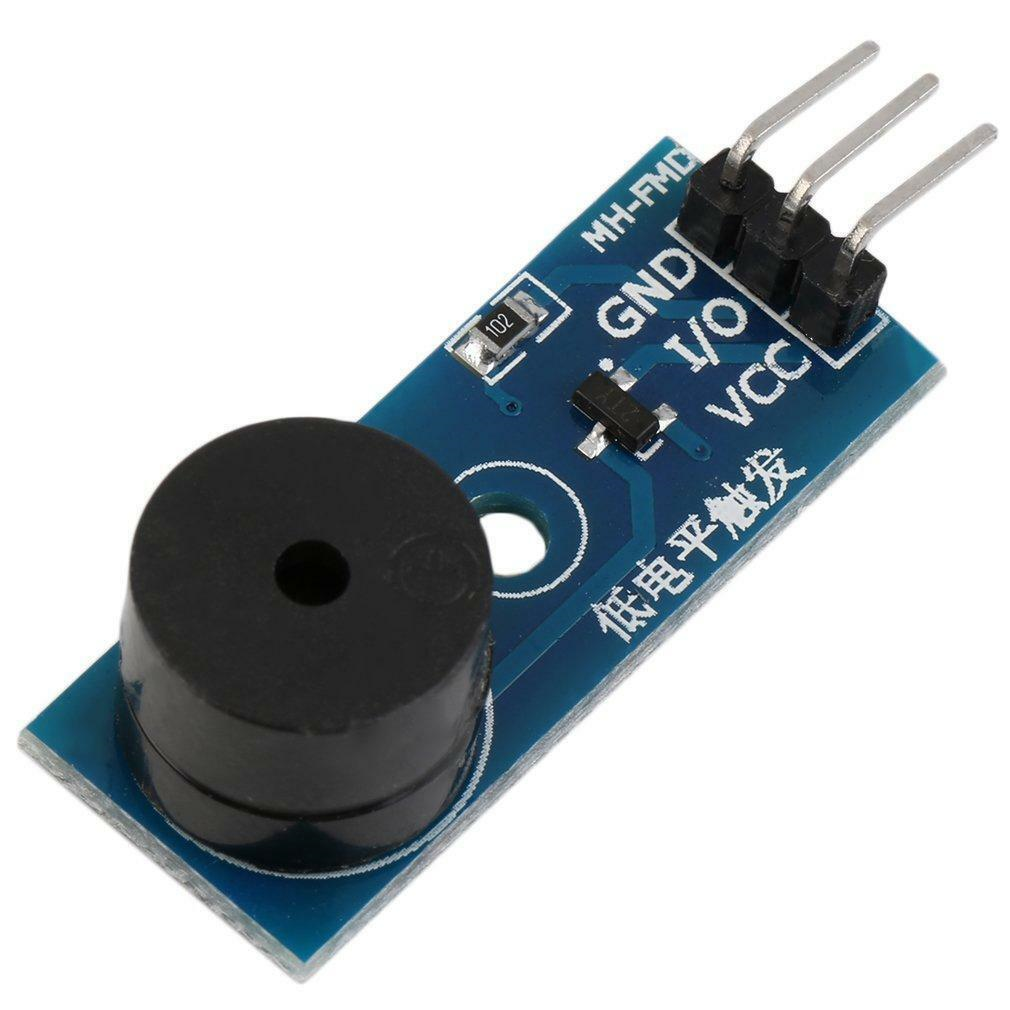
\includegraphics[scale=0.2]{images/buzzer}
\caption{Piezo-električna zujalica} \label{fig:buzzer}
\end{figure}

\vspace{10pt}

\pagebreak

	\subsection{LCD I2C 16x2}
	
	Kao osnovni način prikazivanja merenih vrednosti izabran je LCD 16x2. Pošto se broj slobodnih pinova smanjivao kako su se dodavali novi elementi u projekat, broj od 16 pinova potreban za povetivanje LDC displeja je postao problem. Rešenje ovog problema je bilo spajanje na I2C modul (Slika \ref{fig:I2CLCD}) koji drastično smanjuje broj potrebnih pinova sa 16 na 4. I2C (Inter-Integrated Circuit) je serijski protokol komunikacije koji omogućava digitalnim uređajima da razmenjuju podatke i komande putem dva voda - Serial Data (SDA) i Serial Clock (SCL). Pinovi ovog modula su GND, VCC (5V), SDA i SCL. Arduiono UNO R3 već poseduje SDA i SCL pinove baš za ovu upotrebu, ali se mogu koristiti i ostali analogni pinovi kao npr. pin A4 i A5. Dimenzije LCD-a sa I2C modulom iznose 80x36x19.25mm
	
	\begin{figure}[H]
\centering
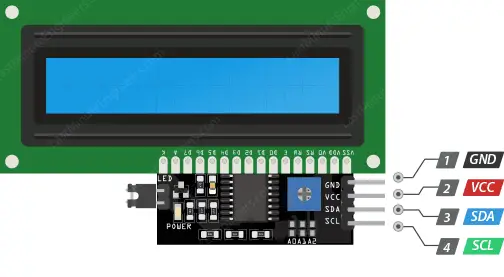
\includegraphics[scale=0.6]{images/I2CLCD}
\caption{LCD 16x2 sa I2C modulon} \label{fig:I2CLCD}
\end{figure}
	


	\subsection{4x4 tastatura}
	
	Poslednji elemenat koji će poboljšati korisničko iskustvo je senzor dodira tj. 4x4 tastatura. Tastatura se sa stoji između dva sloja. Jeden je spoj svih redova, a drugi svih kolini. Pritiskom se pravi kontakt između ova dva sloja čime se i determiniše koji je taster pritisnut. Za sve izabrane funkcionalnosti iskorišćeno je smo prva dva reda i 4 kolone. Tako da od ukupnog broja pinova kojih je 8 ovde se koriste samo 6 (2 za redove i 4 za kolone). Pinovi su spojeni na sledeće portove Arduina C1->D5, C2->D4, C3->D3, C4->D2, R1->D9 i R2->D8. Funkcionalnosti tastera biće objašnjne u sledećem poglavlju.
	
\pagebreak

	\subsection*{Šema kola projekta}
	
\begin{figure}[H]
\centering
\rotatebox{270}{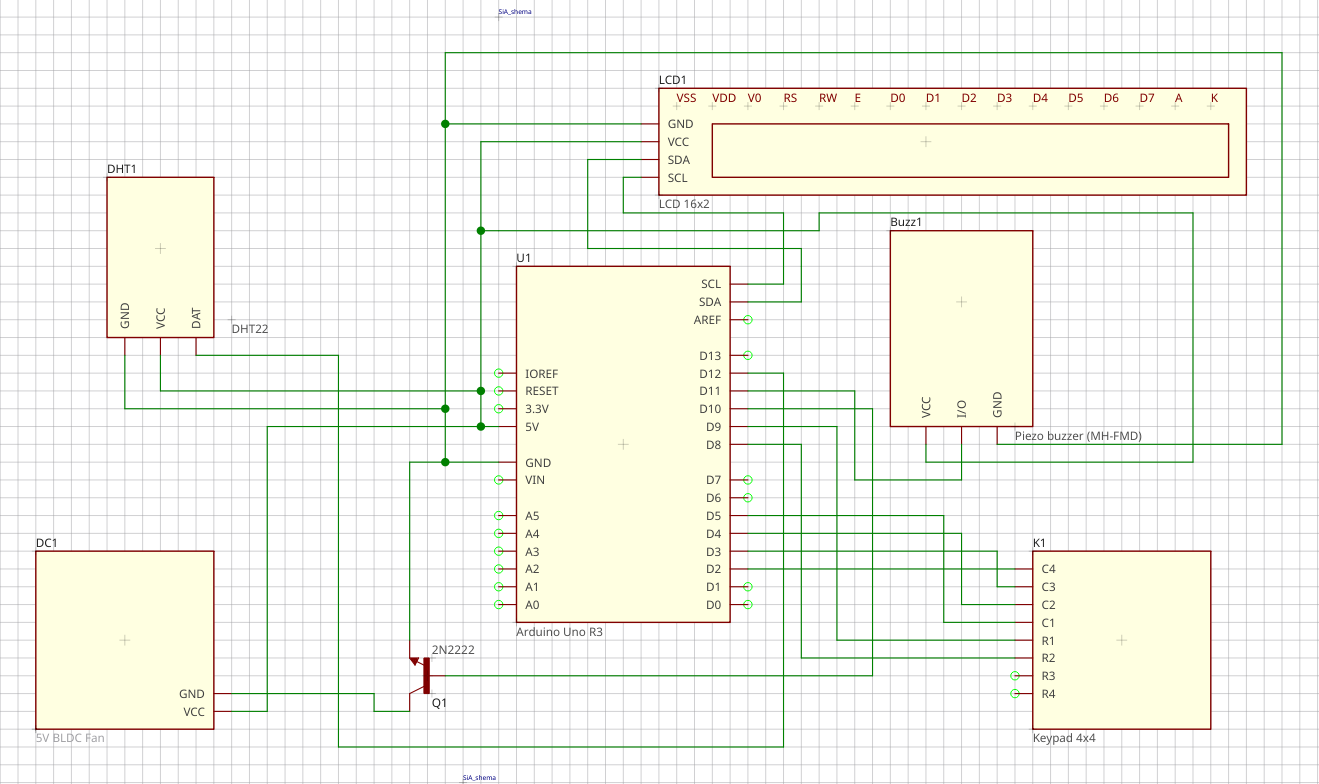
\includegraphics[scale=0.5]{images/circuit_diagram}} 
\label{fig:circuit_diagram}
\end{figure}

\vspace{10pt}

\pagebreak
\endgroup

\begingroup
\sloppy

\section{Softverska realizacija projekta}

\vspace{10pt}

U ovom poglavlju se govori u kratkim crtama o kodu koji pokreće hardver projekta. Kod je izrađen u Arduino okruženju, a nalazi se na \textbf{\texttt{\href{https://github.com/vgalovic/temperature-and-humidity-regulator.git}{Github repozitorijumu}}}. Kod projekta se nalazi u  \textbf{\texttt{\href{https://github.com/vgalovic/temperature-and-humidity-regulator/blob/main/code/code.ino}{code/code.ino}}}. Evo detaljnog objašnjenja korisničkog interfejsa:
 
\begin{enumerate}

	\item \texttt{Tastatura}: Korisnik može koristiti tastaturu sa četiri kolone i dva reda za navigaciju i izbor opcija. Na tastaturi su raspoređeni tasteri od 1 do 8 koji imaju različite funkcije:
	\begin{itemize}
		\sloppypar
		\item Tasteri od 1 do 4 služe za odabir različitih režima rada sistema, uključujući prebacivanje između prikaza temperature/vlažnosti i brzine ventilatora/stanja zvučnog alarma, kao i testiranje brzine ventilatora i zvučnog alarma.
        \item Tasteri 5 i 6 se koriste za uključivanje i isključivanje debug moda i podešavanje prilagođenih parametara za granice vlažnosti i temperature.
        \item Taster 8 se koristi za čišćenje LCD ekrana.
	\end{itemize}
	
	
  	\item \texttt{LCD ekran}: Na LCD ekranu su prikazane različite informacije o sistemu:
  	\begin{itemize}
  		\item Temperatura i vlažnost: Prikazuje se trenutna temperatura u stepenima Celzijusa i vlažnost u procentima.
       	\item Brzina ventilatora i stanje zvučnog alarma: U ovom režimu se prikazuju informacije o brzini ventilatora (izražene u procentima) i stanju zvučnog alarma (uključen ili isključen).
		\item Indikacija Testiranja ventilatora/zvučnog alarma
  	\end{itemize}
  	
  	\item \texttt{ Serijal port}: Dijagnostički podaci u debug modu: Kada je debug mod aktiviran, prikazuju se dijagnostičke informacije preko serijskog porta, dok na LCD ekranu je ispisana brzina prenosa bita po sekundi.
\end{enumerate}

U daljem nastavku poglavalja, biće nabrojane sve biblioteke, makroi, promenljive i funkcije kao i objašnjenje šta oni rade unutar koda.
    
\vspace{10pt}

	\subsection{Biblioteke}
	\begin{itemize}
    		\item \textbf{Keypad}: Koristi se za interakciju sa tastaturom. Github stranica do ove biblioteke je na sledećem \textbf{\texttt{\href{https://github.com/Chris--A/Keypad.git}{linku}}}.
    		
    		\item \textbf{LiquidCrystal\_I2C}: Pomoću nje se kontroliše LCD putem I2C komunikacije. Stranica sajta arduina za preuzimanje biblioteke nalazi se na sledećem \textbf{\texttt{\href{https://downloads.arduino.cc/libraries/github.com/marcoschwartz/LiquidCrystal_I2C-1.1.2.zip}{linku}}}. 
    		
    		\item \textbf{DHT22}: Omogućava čitanje podataka sa DHT22 senzora. Github stranica do ove biblioteke je na sledećem \textbf{\texttt{\href{https://github.com/Chris--A/Keypad.git}{linku}}}.
	\end{itemize}

\newpage

	\subsection{Makroi}

\vspace{10pt}

\begin{enumerate}

	\item \textbf{Pinske Definicije Tastature}:

	\begin{itemize}
    		\item \texttt{R1}, \texttt{R2}: Brojevi pinova za konekciju redova tastature.
    		\item \texttt{C1}, \texttt{C2}, \texttt{C3}, \texttt{C4}: Brojevi pinova za konekciju kolona tastature.
	\end{itemize}

	\item \textbf{Dimenzije Tastature}:
	\begin{itemize}
    		\item \texttt{ROWS}, \texttt{COLS}: Broj redova i kolona u matrici tastature.
	\end{itemize}
	\item \textbf{LCD Konfiguracija}:
	\begin{itemize}
		\item \texttt{I2C\_PORT}: I2C adresa LCD ekrana.
    		\item \texttt{TOTAL\_COLUMNS}, \texttt{TOTAL\_ROWS}: Broj kolona i redova na LCD ekranu.
	\end{itemize}
	\item \textbf{Pinovi}:
	\begin{itemize}
    		\item \texttt{PWM, BUZZ, DHT}: Pinovi za PWM, zvučnik i DHT22 senzor.
	\end{itemize}

	\item \textbf{Koraci Prilagođavanja}:
	\begin{itemize}
    		\item \texttt{HUMIDITY\_STEP}, \texttt{TEMPERATURE\_STEP}: Veličine koraka za prilagođavanje granica vlažnosti i temperature.
	\end{itemize}

	\item \textbf{Debug i Vremenski Parametri}:
	\begin{itemize}
		\item \texttt{DEBUG\_SERIAL\_BAUDRATE}: Brzina prenosa bita po sekundi za serijsku komunikaciju u debug režimu.
		\item \texttt{DEBOUNCE\_TIME}: Vreme debaunsa za tastaturu.
		\item \texttt{BUZZER\_DELAY}: Vreme kašnjenja za zvučnik.
		\item \texttt{DELAY\_IN\_SETUP}: Kašnjenje na kraju \texttt{setup()} funkcije.
		\item \texttt{DHT\_UPDATE\_INTERVAL}: Interval za ažuriranje temperatura i vlažnosti sa DHT22 senzora.
		\item \texttt{FAN\_SPEED\_UPDATE\_INTERVAL}: Interval za ažuriranje brzine ventilatora na osnovu temperature.
	\end{itemize}
	
	
	\item \textbf{Podrazumevane Vrednosti}:
	\begin{itemize}
		\sloppypar
    		\item \texttt{DEFAULT\_HUMIDITY\_MIN}, \texttt{DEFAULT\_HUMIDITY\_MAX},\\ \texttt{DEFAULT\_TEMPERATURE\_MIN}:
    		\\ Podrazumevane minimalne i maksimalne granice vlažnosti i podrazumevana minimalna granica temperature.
	\end{itemize}

\pagebreak

	\item \textbf{Prilagođavanje Vlažnosti i Temperature}:
	\begin{itemize}
    		\item \texttt{HUMIDITY\_MIN\_LOWER\_LIMIT}, \texttt{HUMIDITY\_MIN\_UPPER\_LIMIT}:\\ Donja i gornja granica za prilagođavanje minimalne granice vlažnosti.
    		\item \texttt{HUMIDITY\_MAX\_LOWER\_LIMIT}, \texttt{HUMIDITY\_MAX\_UPPER\_LIMIT}:\\ Donja i gornja granica za prilagođavanje maksimalne granice vlažnosti.
    		\item \texttt{TEMPERATURE\_MIN\_LOWER\_LIMIT}, \texttt{TEMPERATURE\_MIN\_UPPER\_LIMIT}:\\ Donja i gornja granica za prilagođavanje minimalne granice temperature.
	\end{itemize}

	\item \textbf{Koraci Prilagođavanja}:
	\begin{itemize}
    		\item \texttt{HUMIDITY\_STEP}, \texttt{TEMPERATURE\_STEP}: Veličine koraka za prilagođavanje granica vlažnosti i temperature.
	\end{itemize}

\end{enumerate}


	\subsection{Promenljive}

\vspace{10pt}

\begin{enumerate}
    \item \textbf{action\_state}:
        \begin{itemize}
            \item \textbf{Tip}: Enumeracija
            \item \textbf{Opis}: Predstavlja trenutno stanje sistema. Moguća stanja uključuju:
                \begin{itemize}
                    \item \texttt{NORMAL\_DISPLAY}: Normalni prikaz za prikazivanje temperatura i vlažnosti vazdiha ili brzinu ventilatora i stanje zvučnika.
                    \item \texttt{DEBUG\_MODE}: Režim za debagiranje za prikaz dijagnostičkih informacija sa DHT22 senzora.
                    \item \texttt{FAN\_TEST}: Režim za testiranje brzine ventilatora.
                    \item \texttt{BUZZER\_TEST}: Režim za testiranje zvučnika.
                \end{itemize}
        \end{itemize}
        
    \item \textbf{display\_state}:
        \begin{itemize}
            \item \textbf{Tip}: Logička
            \item \textbf{Opis}: Kontroliše da li LCD ekran prikazuje očitavanja temperature i vlažnosti (\texttt{true}) ili brzinu ventilatora i stanje zvučnika (\texttt{false}).
        \end{itemize}
        
    \item \textbf{debug\_enable}:
        \begin{itemize}
            \item \textbf{Tip}: Logička
            \item \textbf{Opis}: Određuje da li je režim za debagiranje omogućen (\texttt{true}) ili nije (\texttt{false}), što omogućava dijagnostičke informacije sa DHT22 senzora.
        \end{itemize}
        
    \item \textbf{humidity\_min}, \textbf{humidity\_max}, \textbf{temperature\_min}:
        \begin{itemize}
            \item \textbf{Tip}: Broj (Unsigned 8-bit integer)
            \sloppypar
            \item \textbf{Opis}: Definiše minimalne i maksimalne pragove vlažnosti (\textbf{humidity\_min}, \textbf{humidity\_max}) i minimalni prag temperature (\textbf{temperature\_min}) za sistem.
        \end{itemize}
        
    \item \textbf{en\_mill}:
        \begin{itemize}
            \item \textbf{Tip}: Unsigned long
            \item \textbf{Opis}: Čuva trenutno vreme u milisekundama za potrebe vremenskog merenja u glavnoj petlji.
        \end{itemize}
\end{enumerate}

\newpage

	\subsection{Funkcije}

\vspace{10pt}

\begin{enumerate}[label=\arabic*.,leftmargin=*]
    \item \textbf{buzzControl(humidity)}:
        \begin{enumerate}[label={},leftmargin=*]
            \item Proverava da li vlažnost pada ispod minimalnog praga ili prelazi preko maksimalnog praga i aktivira zvučnik prema tome. Vraća \texttt{true} ako je zvučnik aktiviran.
        \end{enumerate}
        
    \item \textbf{dcFanControl(temperature)}:
        \begin{enumerate}[label={},leftmargin=*] 
            \item Prilagođava brzinu ventilatora na osnovu temperature. Vraća procenat brzine ventilatora.
        \end{enumerate}
        
    \item \textbf{display()}:
        \begin{enumerate}[label={},leftmargin=*]
            \item Dobavlja očitavanja temperature i vlažnosti vazduha sa DHT22 senzora, kontroliše brzinu ventilatora i stanje zujalice, i prikazuje relevantne informacije na LCD ekranu.
        \end{enumerate}
        
    \item \textbf{debugMode()}:
        \begin{enumerate}[label={},leftmargin=*] 
            \item Prikazuje dijagnostičke informacije sa DHT22 senzora u režimu za debagiranje.
        \end{enumerate}
        
    \item \textbf{action()}:
        \begin{enumerate}[label={},leftmargin=*] 
            \item Vrši akcije na osnovu trenutnog stanja sistema, uključujući prikaz normalnih informacija, ulazak u režim za debagiranje ili izvođenje testova ventilatora i zvučnika.
        \end{enumerate}
        
    \item \textbf{keypadEvent(key)}:
        \begin{enumerate}[label={},leftmargin=*] 
            \item Upravlja događajima tastature i izvodi odgovarajuće akcije na osnovu pritisnutog tastera.
        \end{enumerate}
        
    \item \textbf{setParameters()}:
        \begin{enumerate}[label={},leftmargin=*] 
            \item Omogućava korisnicima postavljanje prilagođenih parametara za pragove vlažnosti i temperature koristeći tastaturu.
        \end{enumerate}
        
    \item \textbf{setup()}:
        \begin{enumerate}[label={},leftmargin=*]
        		\sloppypar
            \item Inicijalizuje sistem, uključujući postavljanje pinova, LCD ekrana i inicijalizaciju parametara.
        \end{enumerate}
        
    \item \textbf{loop()}:
        \begin{enumerate}[label={},leftmargin=*] 
            \item Glavna petlja sistema, gde se akcije vrše periodično na osnovu vremenskih intervala.
        \end{enumerate}
\end{enumerate}

\pagebreak
\endgroup

\begingroup
\justifying
\section{Prikaz uređaja u krajnjem stadijumu izrade}

\vspace{10pt}

U ovom poglavlju je na slici \ref{fig:deviceMockup} prikazan krajnji stadium izrade projekta. Na slici \ref{fig:lcdViewTempHumi} je prikazan primer kako izgleda ispis na lcd ekranu.

\vspace{10pt}

\begin{figure}[H]
\centering
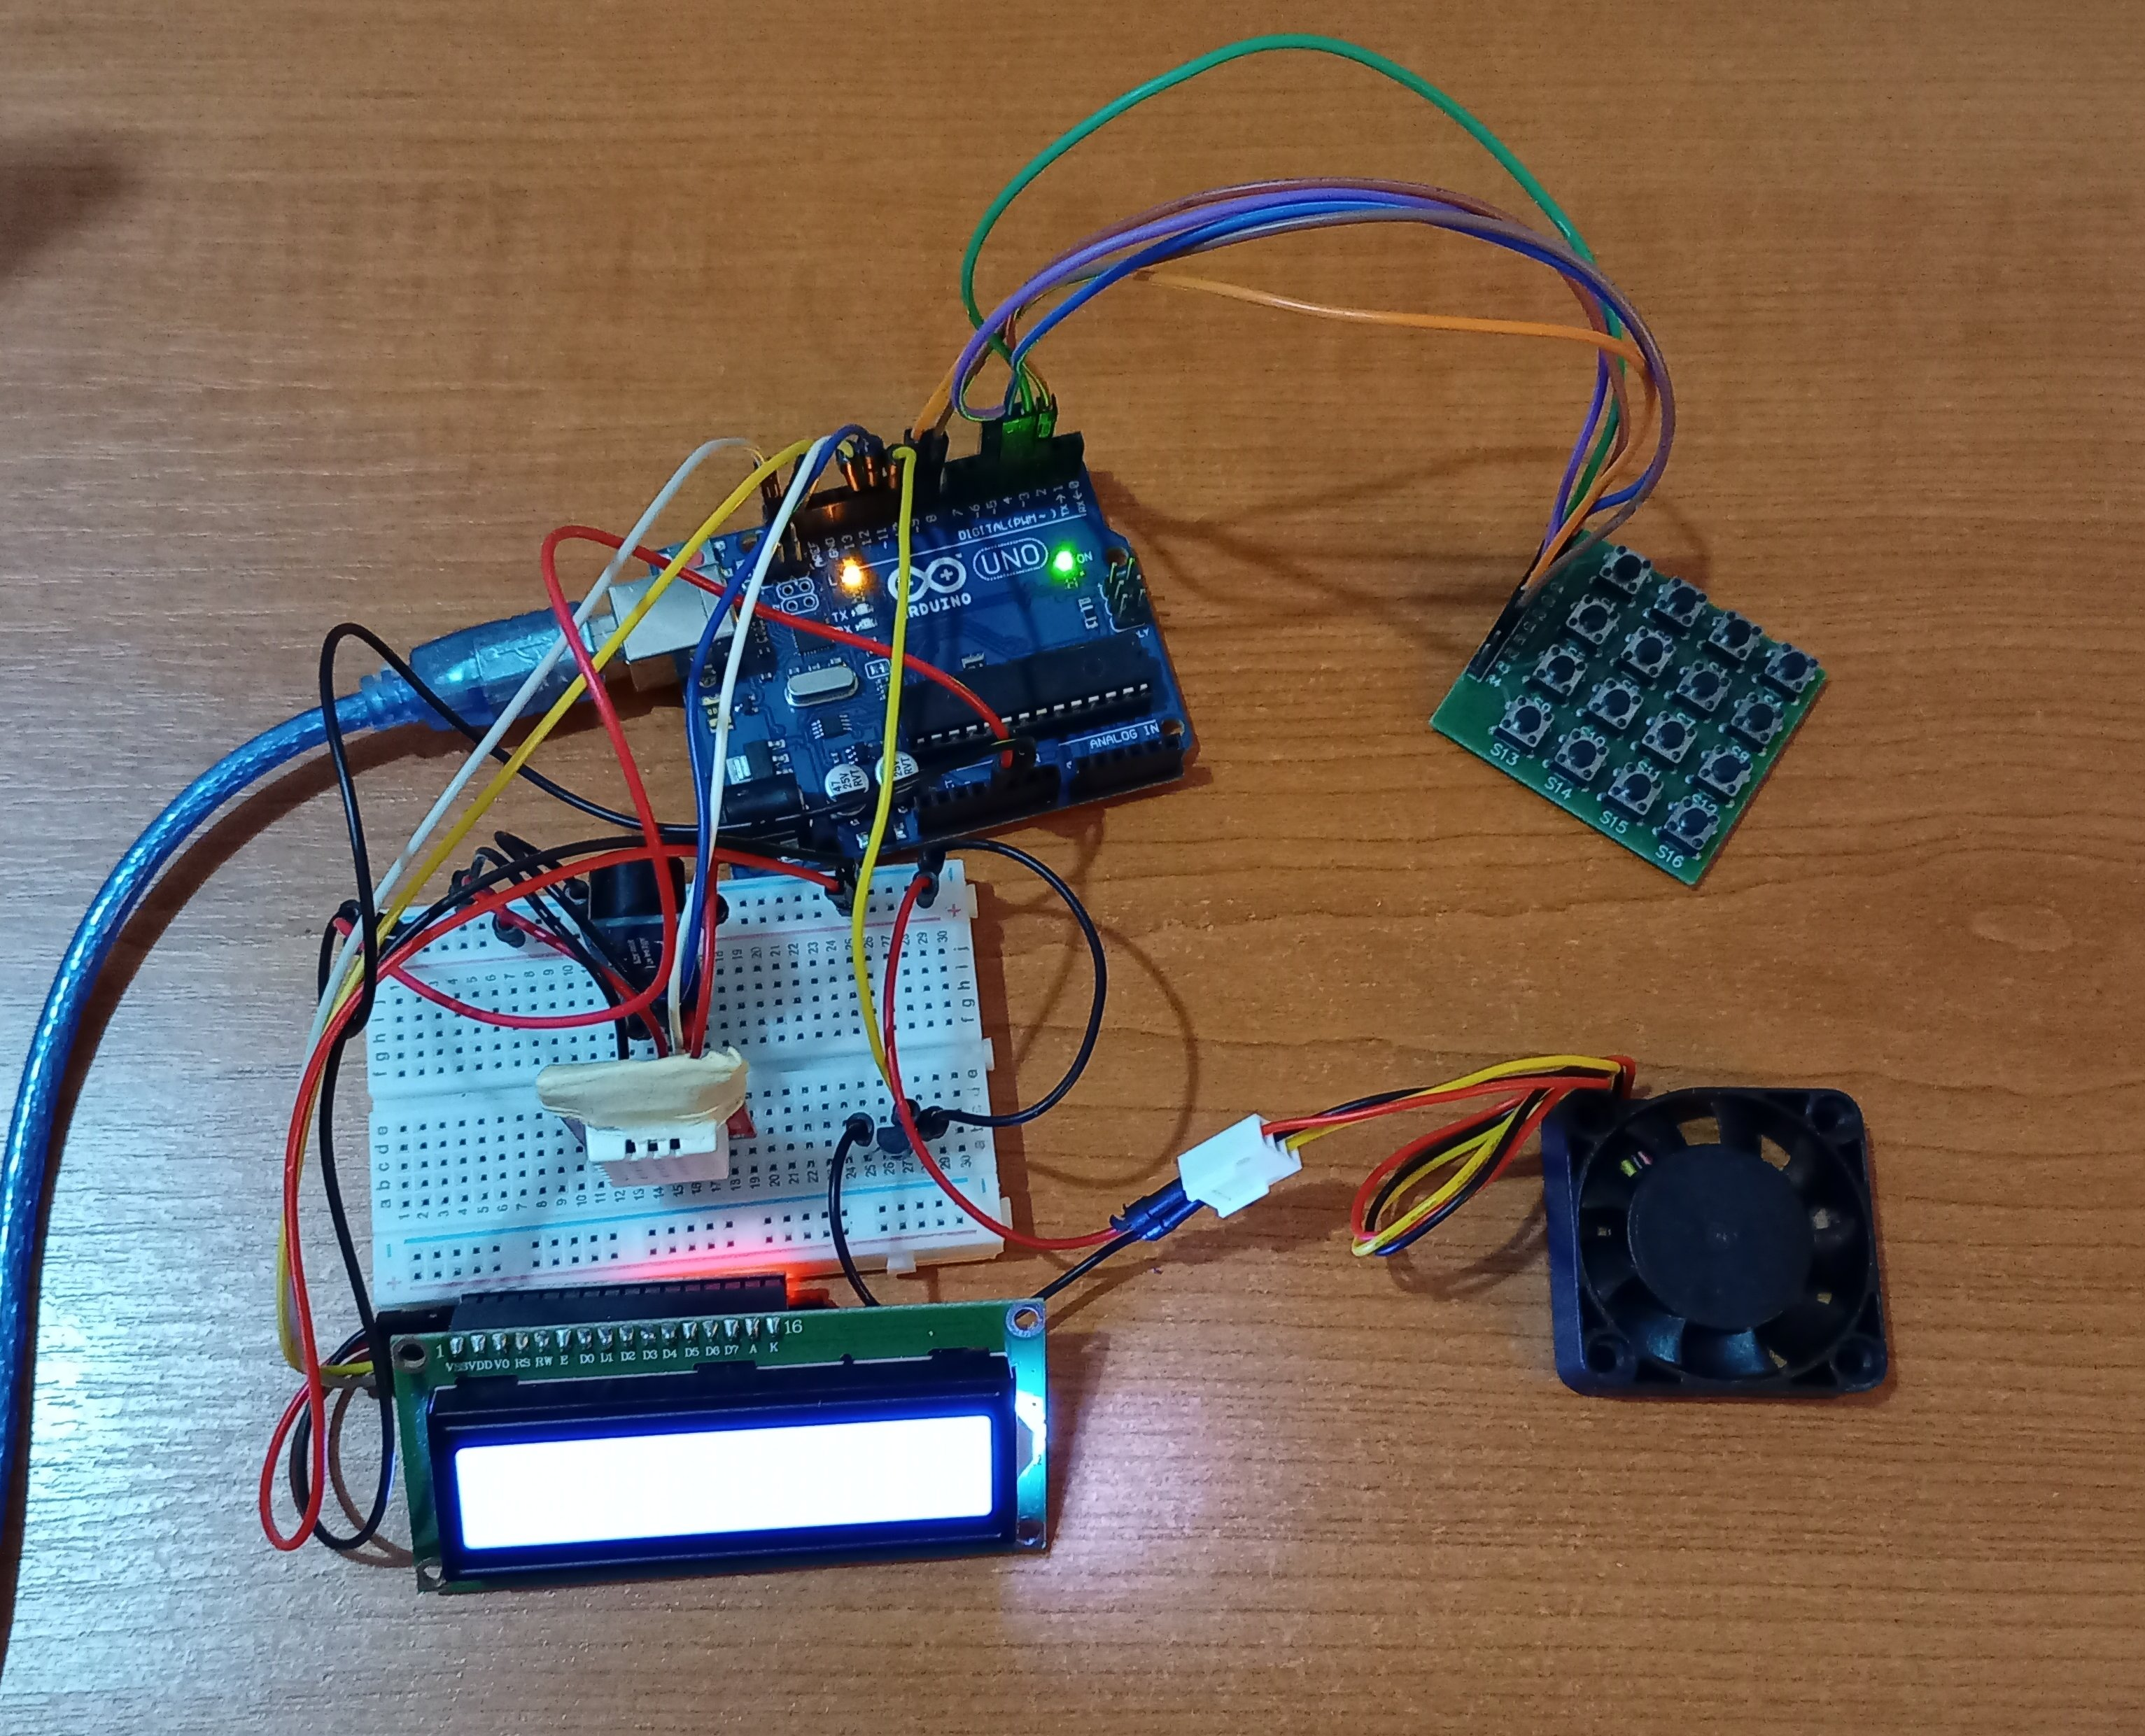
\includegraphics[width=0.8\textwidth]{images/deviceMockup}
\caption{Prikaz uređaja u krajnjem stadijumu izrade}\label{fig:deviceMockup}
\end{figure}

\vspace{10pt}

\begin{figure}[H]
\centering
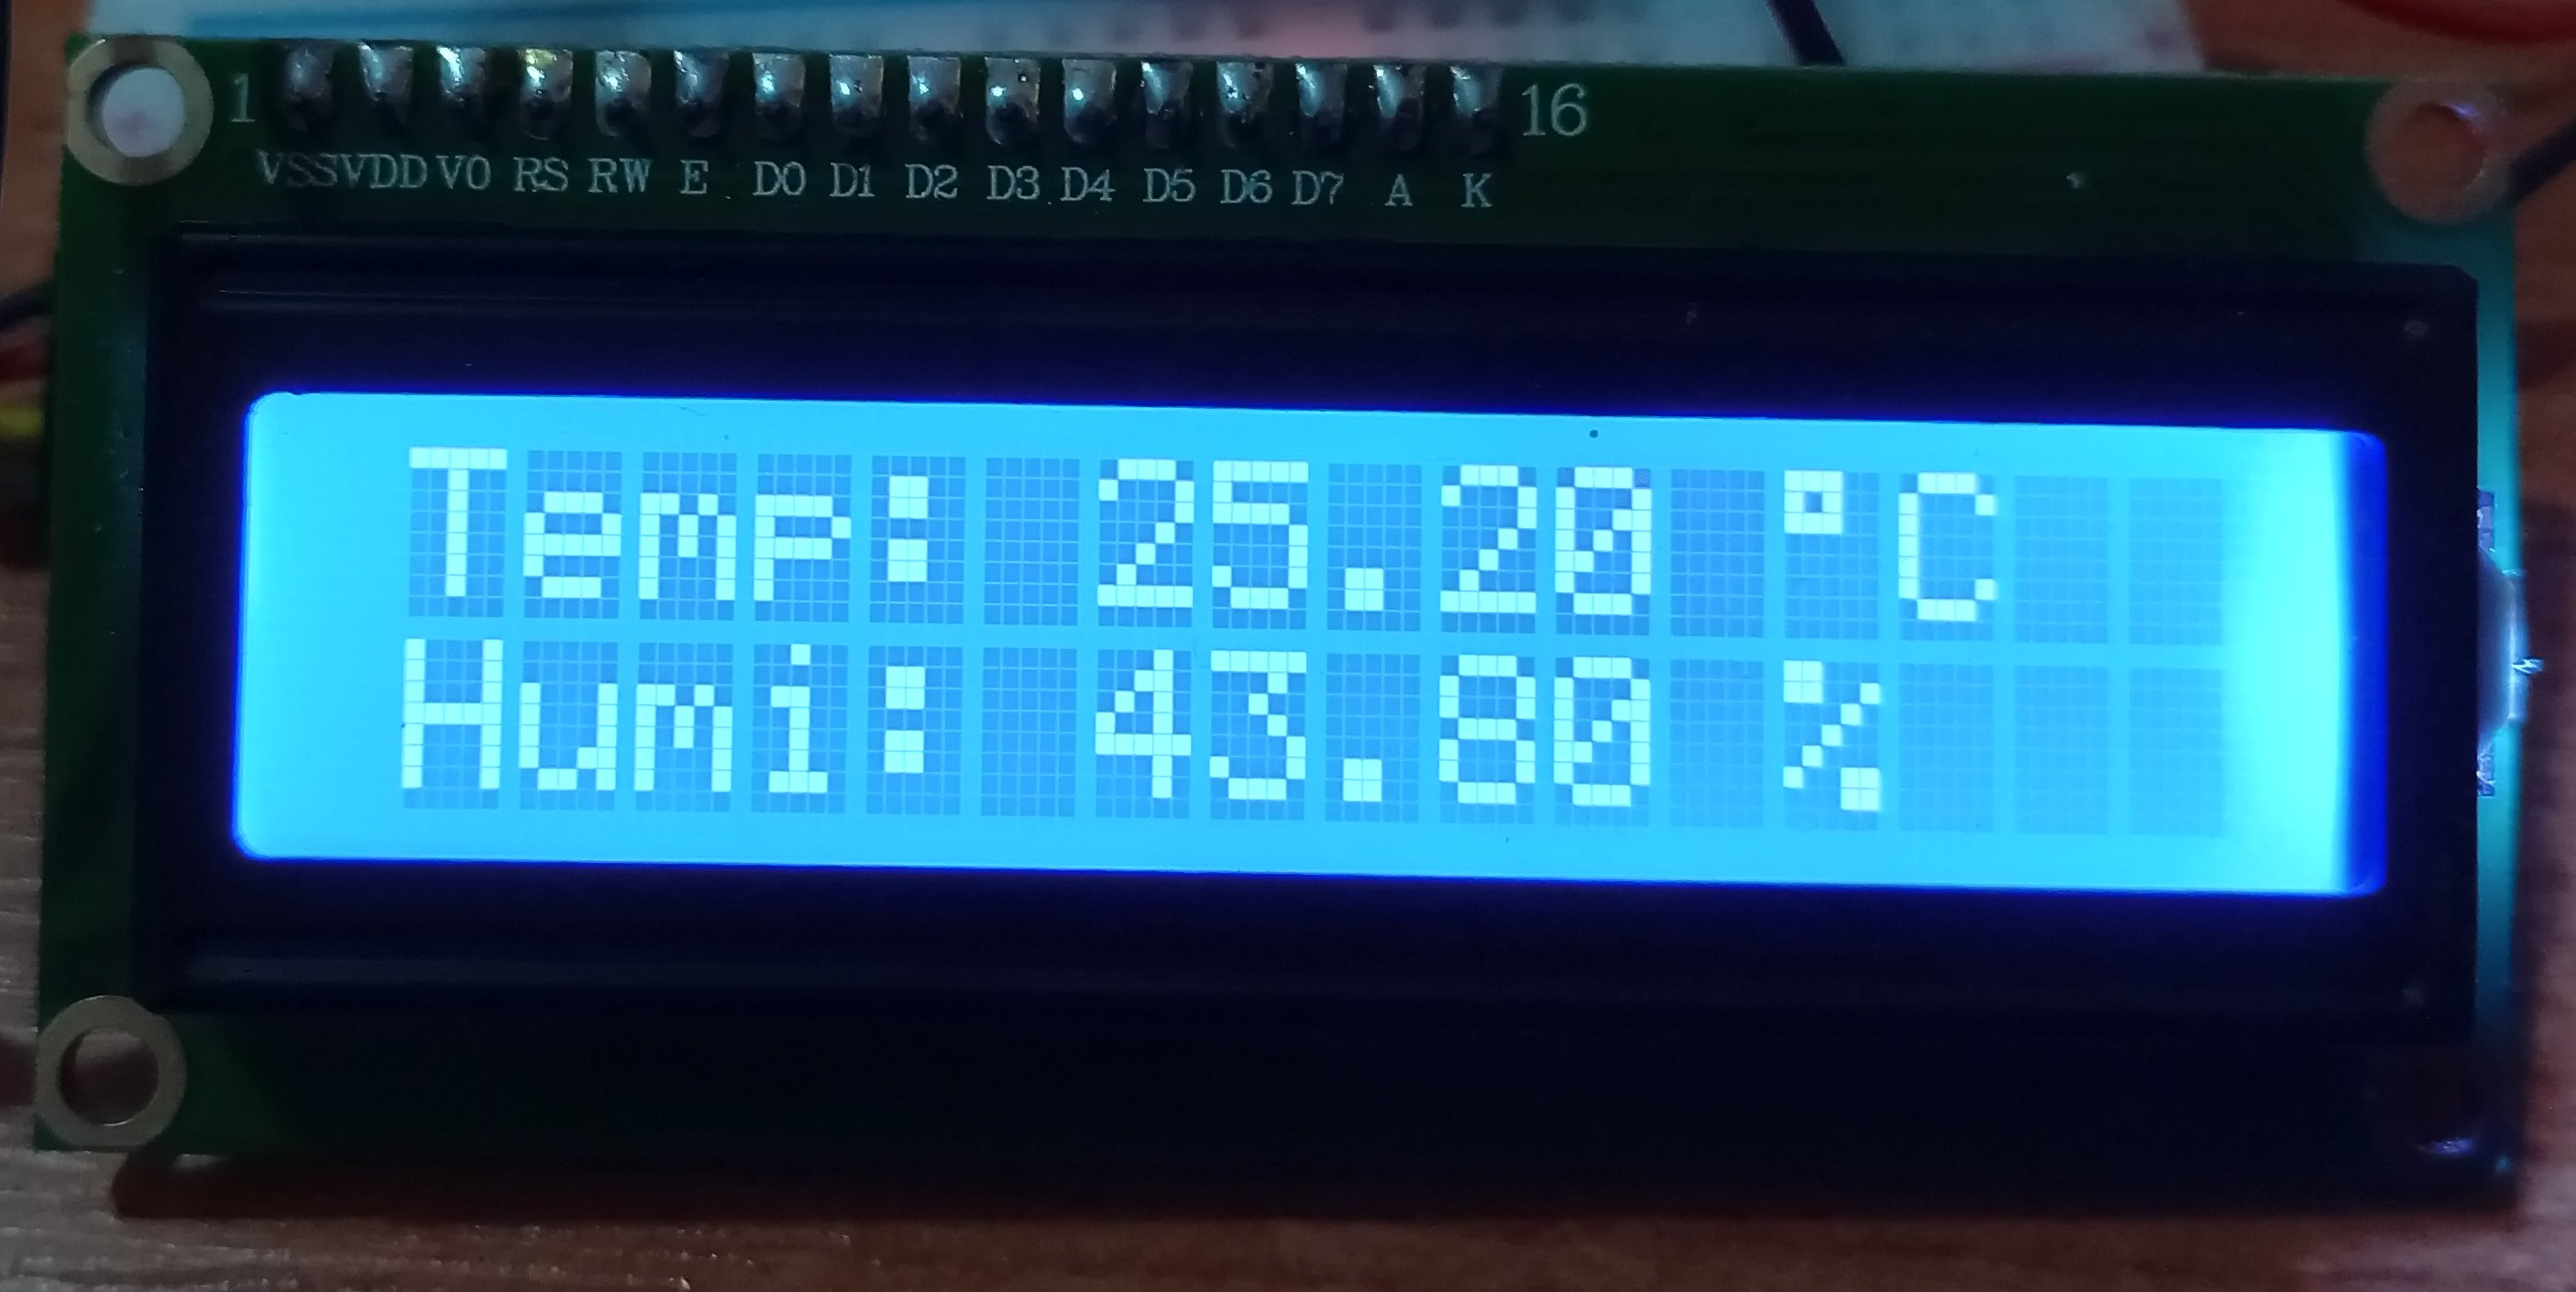
\includegraphics[width=0.8\textwidth]{images/lcdViewTempHumi}
\caption{Prikaztemperatura i vlažnost vazduha na  lcd ekranu}\label{fig:lcdViewTempHumi}
\end{figure}

\endgroup
\pagebreak

\begingroup
\justifying
\section{Rezultati proračuna i testiranja}

\vspace{10pt}


	\subsection{Proračuni BLDC motora }
	
\vspace{10pt}
	
Iako se u projektu koristi BLDC motor, zbog jednostavnijeg proračuna izabran je BDC koji je najbliži po svojim karakteristikama. Motor koji je za to izabran je Maxon A-max 22 od 4.5 V \ref{lib:A-max-22}. Cilj proračuna je računanje odziva brzine vratila motora uz dodatno opterećenje koju stvara propeler ventilatora koji će biti aproksimiran kao disk poluprečnika 20mm i debljine 10mm. Za masu tog diska uzeta je vrednost 2 grama. Primer zadatka koji je najblži narednom proračunu se može pronaći u Zbirci rešenih zadataka iz aktuatora, Damir Krlješ, Zadatak 5 \ref{lib:workbook}.

\vspace{10pt}

Pre određivanja odziva brzine vratila motora moramo izračunati veličine koje nemamo. Prva ta veličina je moment inercije diska (propelera) (\ref{eq:J_disk})

\vspace{10pt}

Ukupan moment inercije:

\begin{align} 
& J_{disk} = \frac{r^2 m_{diska}}{2}=4 \times 10^{-7} kgm^2 \label{eq:J_disk} \\
& J_{motora} = 4.07 \times 10^{-7} kgm^2 \nonumber \\
& J_{uk} = J_{diska} + J_{motora} = 8.07 \times 10^{-7} kgm^2 \nonumber
\end{align}
	
\vspace{10pt}

Sledeća veličina je koeficijent viskoznog trenja koji koji slično inerciji postoji i u motoru i u disku. Takođe pretpostavićemo da naše napajanje nema strujni limit. Koristićemo jednačinu iz mehaničkog modela DC motora koja predstavlja zavisnost brzine vratila i momenta koja deluju na vratilo motora (\ref{eq:M}).

\vspace{10pt}

Koficijent viskoznog trenja:

\begin{align}
M = M_{op} + B \times \omega + \partial \frac{d \omega}{dt} \label{eq:M}
\end{align}

U ustaljenom stanju : $\partial \frac{d \omega}{dt} = 0$

\begin{align*}
M = M_{op} + B \omega
\end{align*}

U praznom hodu : $M _{op} = 0$

\begin{align*}
& M = B \omega\\
& M= k_t I_A\\
& k_t I_A = B_{motora} \omega \\
& B_{motora} = \frac{k_t I_A}{\omega} \\ 
& B_{motora} = 0.209 \times 10^{-6} \frac{Nms}{rad}\\
& B_{diska} = 0.205 \times 10^{-6} \frac{Nms}{rad} \\
& B_{uk} = B_{motora} + B_{diska} = 0.414 \times 10^{-6} \frac{Nms}{rad}
\end{align*}

Krajnja ugaona brzina zavisi od opterećenja i dobija se izjednačavanjem svih momenata koji deluju na vratilo motora kada se on obrće konstantnom brzinom (ubrzanje je nula) (\ref{eq:M_EM}).

\begin{align}
& M_{EM} = M_M \label{eq:M_EM} \\
& k_tI = B_{uk} \omega_{m_\infty} \nonumber \\
& k_t \frac{U-E}{R} = B_{uk} \omega_{m_\infty} \nonumber \\
& k_t \frac{U}{R} - k_t \times k_v \frac{\omega_{m_\infty}}{R} =  B_{uk} \omega_{m_\infty} \nonumber \\
& \omega_{m_\infty} = \frac{U}{ k_v + \frac{B_{uk} \times R}{k_t} } = 747.42 \frac{rad}{s} \nonumber
\end{align}


\vspace{10pt}


Za proveru određene brzine obrtanja motora izabrana je simulaciju u Simuliku koja pored odziva prikazuje trenutak kada motor izlazi iz strujnog limita ($T_{s\_limit} \approx 0.15$s). Možemo videti da je krajnja brzina motora na grafiku približna prethodo izračunatoj brzini (Grafik \ref{grafiik:step_response}).

\vspace{10pt}

\begin{grafik}
\begin{center}
\begin{tikzpicture}
\centering
\begin{axis}[width=\linewidth, height=10cm,
	xlabel={Vreme [s]},    
    ylabel={Amplituda},
    label style={font=\small},
    xmin=0, xmax=0.25,
	scaled x ticks=false,
	xticklabel style={/pgf/number format/fixed,},
    %xtick={0, 0.05, 0.1, 0.15, 0.2, 0.25},
	ymin=0, ymax=800,
    legend pos=north west,
    ymajorgrids=true,
    grid style=dashed]
     
\addplot[no marks, color=blue] table[x=Time, y=Amplitude]{step_response/step_response.txt};

\addplot[mark=*, color=red] coordinates{(0.1497, 731.2692)} node[pin=-30:{$T_{s\_limit}	\approx 0.15$s}]{};
\draw [dashed,help lines, color=red] (0,731.2692) -| (0.1497,0);

\end{axis}
\end{tikzpicture}
\end{center}			
\caption{Odziv brzine vratila motora}\label{grafiik:step_response}
\end{grafik}

\pagebreak


	\subsection{Testiranja senzora DHT22}
	
\vspace{10pt}

Za testiranje senzora su izabrane metode koje bi bile lake za ponovnu reprodukciju u kućnim uslovima. Pretpostavljeno je da radi testiranja krejnjih vrtednosti temperature i vlažnosti vazduha DHT22 senzora treba obaviti odvojena testiranje tih vrednosti. 

		\subsubsection*{Testiranje merenja vlage senzora DHT22}

\vspace{10pt}	
		
Testiranje vlage zatvorene sredine je sprovedeno lepljenjem DHT22 za unutrašnju stranu poklopca plastične kutije. Na dno plastične kutije zapremine 1650ml je sipano 250ml vode na različitim temperaturama. Počevši od sobne temperature od 25°C pa sve do 55°C. Poklopcem sa senzorom zatvaramo kutiju i merimo vrednosti relativne vlažnosti vazduha (Slika \ref{fig:testHumi}).

\vspace{10pt}

\begin{figure}[H]
\centering
\rotatebox{270}{\includegraphics[scale=0.09]{images/testHumi}}
\caption{Slika testiranja merenja vlage senzora DHT22} \label{fig:testHumi}
\end{figure}

\pagebreak

\sloppypar
Primećeno je da su mala povećanja temperature vode imala veliki uticaj na brzinu povećanja merene vlage vazduha (Grafik \ref{grafik:humi}). Na temperaturi vode od 55°C izmerena vlaga je dostigla svoj maksimum za 22 sekunde, dok se temperatura vazduha promenila za svega 2-3°C čime je potvrđena prethodna pretpostavka za odvojeno merenje vrednosti senzora. Na većim temperaturama (45°C i 55°C) merenje je i prekinuto zbog opreznosti da kondenzacija vode u kućištu senzora ne napravi grešku i zbog već brzog dolaska do 100\% relativne vlažnosti vazduha.

\vspace{10pt}


\vspace{10pt}

\begin{grafik}	
\begin{center}
\begin{tikzpicture}
\centering
\begin{axis}[width=\linewidth, height=12cm,
    xlabel={Vreme [s]},
	ylabel={Vlažnost [\%]},        
    label style={font=\small},
	xmin=2, xmax=40,    
    ymax=100,
    legend pos=north west,
    ymajorgrids=true,
    grid style=dashed]
     
\addlegendentry{Voda: 25.0 °C}
\addplot[no marks, color=blue] table[x=Time, y=Humidity]{tests/humidity/test1.txt};

\addlegendentry{Voda: 30.0 °C}
\addplot[no marks, color=green] table[x=Time, y=Humidity]{tests/humidity/test2.txt};

\addlegendentry{Voda: 35.0 °C}
\addplot[no marks,  color=yellow] table[x=Time, y=Humidity]{tests/humidity/test3.txt};

\addlegendentry{Voda: 45.0 °C}
\addplot[no marks,  color=orange] table[x=Time, y=Humidity]{tests/humidity/test4.txt};

\addlegendentry{Voda: 55.0 °C}
\addplot[no marks,  color=red] table[x=Time, y=Humidity]{tests/humidity/test5.txt};

\end{axis}
\end{tikzpicture}
\end{center}	
\caption{Testiranja merenja vlage senzora DHT22} \label{grafik:humi}
\end{grafik}

\pagebreak

		\subsubsection*{Testiranje merenja temperature senzora DHT22}

\vspace{10pt}		
		
Testiranje temperature nije izvršeno u zatvorenoj sredini zbog izbora kuhinjskog rešoa za grejno telo. Pretpostavljeno je da bi veličina i jačina ovog grejnog tela prebrzo zagreja bilo koji materijal poput prethodno korišćene plastične kutije. Temperaturu smo merili u dve verzije eksperimenta:
	
	\begin{enumerate}[label={\alph*)}]
		\item Kada je TP-300 direktno prislonjen na grejno telo,
		\item Kada je TP-300 na istoj visini kao i DHT22.
	\end{enumerate}


		\subsubsection*{a) Testiranje merenja temperature kada je TP-300 direktno prislonjen na grejno telo}

Senzor je hvataljkom postavljen na visinu od 60mm iznad centra rešoa (Slika \ref{fig:testTempA}), a referentna temperatura samog rešoa merena je kuhinjskim termometrom TP-300 \ref{lib:TP300}.

\vspace{10pt}

\begin{figure}[H]
\centering
\rotatebox{90}{\includegraphics[scale=0.09]{images/testTempA}}
\caption{Slika testiranja merenja temperature senzora DHT22} \label{fig:testTempA}
\end{figure}

\pagebreak

Iz testiranja je primećeno da za široku promenu merene temperature na senzoru potrebne su velike temperature grejnog tela (rešoa). Inegracija grejnog tela u sam projekat bi kompromitovala mnoge plastične komponente korišćene u projektu uzeći u obzir da je temperatura na kojoj se PVC plastika deformiše je 40-80°C. Krajnja vrednosti koju je senzor, koji poseduje plastično kućište, izmerio je bila 65°C dok je vrednost grejnog tela bila 184°C (Grafik \ref{grafiik:tempB}). Time je potvrđena pretpostavka u Uvodu da se izbacivanjem grejnih elemenata projekat drastično pojednastavljuje. 

\vspace{10pt}

\begin{grafik}
\begin{center}
\begin{tikzpicture}
\centering
\begin{axis}[width=\linewidth, height=8cm,
	xlabel={Vreme [s]},    
    ylabel={Temperatura [°C]},
    label style={font=\small},
    xmin=2, xmax=650,
	ymax=200,
    legend pos=north west,
    ymajorgrids=true,
    grid style=dashed]
     
\addlegendentry{DHT22}
\addplot[no marks, color=blue] table[x=Time, y=Temperature]{tests/temperature/testA1.txt};

\addlegendentry{Kuhinjski termometar(TP300)}
\addplot[no marks, color=red] table[x=Time, y=Temperature]{tests/temperature/testA2.txt};

\end{axis}
\end{tikzpicture}
\end{center}			
\caption{Testiranja merenja temperature senzora DHT22}\label{grafiik:tempA}
\end{grafik}

\pagebreak

	\subsubsection*{b) Testiranje merenja temperature kada je TP-300 na istoj visini kao i DHT22}

\vspace{10pt}		
		
Senzor je ostao na istoj visini od 60mm iznad centra rešoa (Slika \ref{fig:testTempB}), a kuhinjski termometar TP-300 je postavljen na istu distancu od rešoa kao i senzor.\ref{lib:TP300}.

\vspace{10pt}

\begin{figure}[H]
\centering
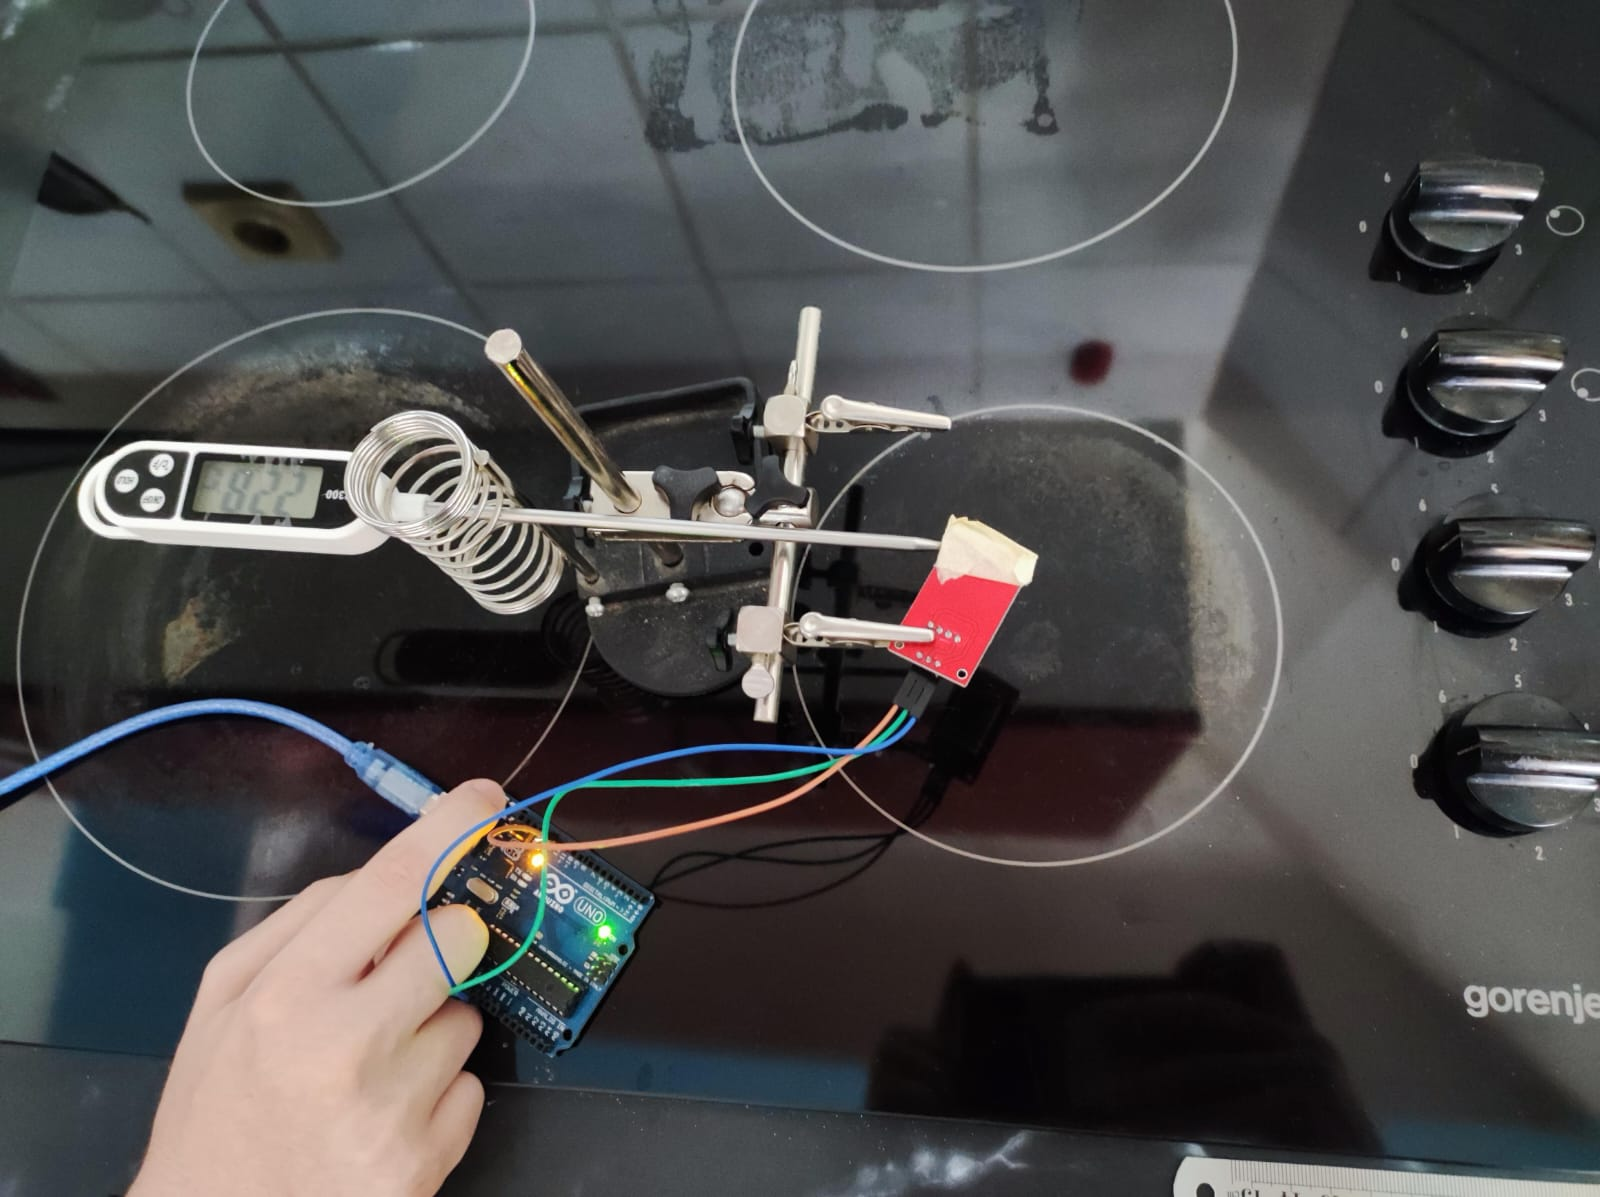
\includegraphics[scale=0.25]{images/testTempB}
\caption{Slika testiranja merenja temperature senzora DHT22} \label{fig:testTempB}
\end{figure}

\pagebreak

Iz ovog testiranja je primećeno da kuhinjski termometar, i ako izabran za referentnu tačku, primetno kasni za senzorom DHT22. Razlog za ovaku razliku možemo uzeti osnovne primene ova dva merna uređaja. DHT22 je namenjen za merenje temperature i vlažnosti vazduha, dok je kuhinjski termometar TP300 namenjen za kontaktno merenje temperature neke tečnosti ili hrane. Površina je još jedan moguću faktor koji je uticao na ovakav rezultat jer je očigledna veća površina DHT22 od TP300.

\vspace{10pt}

\begin{grafik}
\begin{center}
\begin{tikzpicture}
\centering
\begin{axis}[width=\linewidth, height=8cm,
	xlabel={Vreme [s]},    
    ylabel={Temperatura [°C]},
    label style={font=\small},
    xmin=2, xmax=650,
	ymax=100,
    legend pos=north west,
    ymajorgrids=true,
    grid style=dashed]
     
\addlegendentry{DHT22}
\addplot[no marks, color=blue] table[x=Time, y=Temperature]{tests/temperature/testB1.txt};

\addlegendentry{Kuhinjski termometar(TP300)}
\addplot[no marks, color=red] table[x=Time, y=Temperature]{tests/temperature/testB2.txt};

\end{axis}
\end{tikzpicture}
\end{center}			
\caption{Testiranja merenja temperature senzora DHT22}\label{grafiik:tempB}
\end{grafik}


\pagebreak
\endgroup

\begingroup
\sloppy
%\justifying
\section{Zaključak}

\vspace{10pt}

Osnovni zadatak ovog projekta je regulisanje temperature i vlažnosti vazduha u nekoj zatvorenoj sredini poput humidora. Odstupanja su nastala kako bi olakšala određene elemente projekta. Jedno odstupanje je nastalo pri aproksimaciji BLDC motora kao BDC motora kako bi se proračun pojednostavio i izbegla elektronska komutacija BLDC motora. Drugo od thih odstupanja se odnosilo na testiranje merenja temperature senzora DHT22 jer se merenje nije vršilo u zatvorenoj sredini kako ne bi došlo do oštećenja senzora ili nezgode zbog visoke temperature.

\vspace{10pt}

Komponenta koja je osnova ovog projekta je senzor temperature i vlažnosti vazduha DHT22. Oko njega je ostatak projetka smišljen i realizovan. Za uređaj koji bi koristio merene vrednosti ovog senzora je izabran primer humidora. To je proširilo raspon ovog projekta ne samo na rad sa senzorom već sistem merenja i regulisanja ovih vrednosti. Izbor ostalih komponenti nastaje kao zadovoljavanja svih funkcionalnosti ovog proširenog sistema. Arduino platforma kao kontrolna jedinica, BLDC motor kao aktuator i osnovi elemenat regulacije, zujalica kao vid zvučnog upozorenja i LCD i 4x4 tastatura za komunikaciju sa korisnikom. Kroz softversku realizaciju je izvršena implementacija svih potrebnih funkcionalnosti poput biranja različitih režima rada i njihovog prikazivanja. Proračuni za aktuator su pored dosta aproksimiranja rezultirali u manje više očekivane vrednosti. Za testiranje senzora su izabrani eksperimenti koji bi najviše odgovarali merenim vrednostima.

\vspace{10pt}

Merenje i regulacija temperature i vlažnosti vazduha neke zatvorene sredine je jedan veoma komplikovan sistem koji zahteva dobru povezanost svih hardverskih i softverskih elemenata.

\vspace{10pt}

Za potencijalno proširenje ovog projekta mogu se dodati dodatni elementi poput grejača koji bi proces regulacije temperature, koji se ovde vrši samo kroz ventilator, proširili. Isto tako bi se mogao dodati i neki izvor dodatne vlažnosti koja bi bila kontrolisana pomoću pumpe. Tada bi se u svim procesima testiranja mogla implementirati zatvorena sredina bez ograničenja, čime bi regulator temperature i vlažnosti vazduha bio potpun. 

\pagebreak
\endgroup

\begingroup
\sloppy

\section{Literatura}

\vspace{10pt}

\begin{enumerate}[label={[\arabic*]}, leftmargin=2.5cm]
	\item Datasheet od DHT22: \label{lib:DHT22-datasheet}\\ \url{https://cdn-shop.adafruit.com/datasheets/DHT22.pdf}
	\sloppypar
	\item Datasheet za Teromometar TP300: \label{lib:TP300}\\ \url{https://dpstar.com.my/wp-content/uploads/2020/04/ecostar-TP-300-Series-Need-Probe-Digital-Thermometer\%E2\%80\%93Dpstargroup.pdf}
	\item Datasheet za A-max 22, 4.5V: \label{lib:A-max-22}\\ \url{https://www.maxongroup.com/medias/sys_master/root/8881643913246/EN-21-168.pdf}	
	\item Damir Krlješ, Zbirka rešenih zadataka iz aktuatora \label{lib:workbook}
\end{enumerate}
\renewcommand{\theenumi}{\arabic{enumi}}

\pagebreak
\endgroup

\end{document}